\lab{Complex Integration}{Integration in the Complex Plane Part 2}{Integration in the Complex Plane Part II}

\objective{Apply Residues to Integration in the Complex Plane}

As we noted in the last lab, there are some important links between the residues of a rational function and its partial fraction decomposition.
Here we will discuss the connection between residues and integrals along the real line and we will also discuss some important applications of residues.

\section*{Evaluating Residues Using Limits and Derivatives}
Often it is faster to evaluate a residue using limits instead of its direct integral definition.
To see how this might be done, consider some function $f$ with a pole of order $1$ at $z_0$.
We say $f$ has a pole of order $n$ at $z_0$ if the first nonzero term in the Laurent Series expansion of is the term corresponding to $(z-z_0)^{-n}$. In the case of our pole of order 1, we then have
$$f(z)=c_{-1}(z-z_0)^{-1}+c_0 (z-z_0)^{0} +c_1 (z-z_0) + \dots$$
So,
$$f(z)(z-z_0)=c_{-1}+c_0 (z-z_0) + c_1 (z-z_0)^2 + \dots$$
Since the right hand side of the Laurent series converges within some nonzero distance of $z_0$, this series will also converge on that domain.
It is an ordinary power series, so it will also be continuous on that domain (it will actually be analytic, but continuity is sufficient here).
This means that we may take the limit of this expression as $z$ approaches $z_0$.
Taking this limit, the only nonzero term of the series remaining is $c_{-1}$, so we have
\begin{equation*}
\lim_{z\to z_0} f(z)(z-z_0) = c_{-1} = \Res{z=z_0} f(z)
\end{equation*}
Now for some $f(z)$ with a pole of order $n$ at $z_0$ we have that within some nonzero distance of $z_0$, the Laurent series of $f$ converges and is of the form
$$f(z)=c_{-n}(z-z_0)^{-n}+\dots+c_0+c_1(z-z_0)+\dots$$
Multiplying by $(z-z_0)^{n}$ and differentiating $n-1$ times, we have
$$\frac{d^{n-1}}{dz^{n-1}}(f(z)(z-z_0)^{n})=(n-1)! c_{-1} + \frac{n!}{1!} c_0 (z-z_0) + \frac{(n+1)!}{2} c_1 (z-z_0)^2!+\dots$$
Taking the limit, we have
\begin{equation*}
\lim_{z\to z_0}\frac{d^{n-1}}{dz^{n-1}}((z-z_0)^n f(z)) = (n-1)! c_{-1}
\end{equation*}
Which implies
\begin{equation*}
\Res{z=z_0}f(z)=\frac{1}{(n-1)!}\lim_{z\to z_0}\frac{d^{n-1}}{dz^{n-1}}((z-z_0)^n f(z))
\end{equation*}
Another useful trick involving poles and residues involves the logarithmic residue, i.e. the residue of the logarithmic derivative $\frac{d}{dz}(\ln(f(z))) = \frac{f'(z)}{f(z)}$.
A natural consequence of the Laurent series expansion of $f(z)$ and $f'(z)$ at a pole $z_0$ is that, where $d$ is the degree of the pole at $z_0$ is that
\begin{equation*}
- \Res{z=z_0} \frac{f'(z)}{f(z)} = d
\end{equation*}
This is a useful bit of information that may be used to simplify computation of residues or of the Laurent series expansion of a function. 
Another way we can evaluate residues is by the following theorem.
\begin{theorem}
Let $f(z)=\frac{p(z)}{q(z)}$ and let $p$ and $q$ be holomorphic at $z_0$. Let $p(z_0) \neq 0$ and $q(z_0)=0$. Suppose that $z_0$ is a pole of order $1$ of $f$. Then 
\begin{equation*}
\Res{z=z_0} f(z) = \frac{p(z_0)}{q'(z_0)}
\end{equation*}
\end{theorem}

\begin{problem}
Write a Python function that given a function and one of it's poles uses \li{sympy.residue} to calculate the order of that pole and with that information calculate the residue of the function using symbolic limits and derivatives. Verify that your function calculates the correct order and check the residue against \li{sympy.residue}, using the function
$$f(z) = \frac{1}{(z^+1)^{4}(2z+1)}dz$$
(The roots are somewhat obvious here, but as a note you can use \li{sympy.solve} to find the roots).
\end{problem}

\begin{comment}This is a big long of a problem with many parts
\begin{problem}
Write a python function, which, using symbolic integration in SymPy, returns the Laurent series expansion of a function about a given pole.
Use the trick involving logarithmic residues to figure out what the degree of the pole is, then use symbolic limits and derivatives to compute the coefficients of the corresponding Laurent series expansion (look at the original equation for the coefficients of the Laurent Series and see that they can be rewritten as residues).
You may assume that the pole is not an essential singular point.
(Recall that, as we defined it, a pole is not an essential singular point, so it will always have a finite degree).
\end{problem}
\end{comment}

\begin{problem}
Write a function which uses SymPy to evaluate the residue of a function $f(z)$ at a plot $z=z_0$ in the case that: $f(z)$ may be written as the quotient of two functions analytic everywhere within some nonzero distance of $z_0$ and the pole of $f(z)$ at $z_0$ is of order $1$.
Test out your function by finding the residues of all the six distinct, order 1 poles of 
$$\frac{z^2}{z^6+1}dz$$
\end{problem}

\section*{Evaluating Indefinite Integrals Using Residues}

One convenient use of residues is the evaluation of integrals that are difficult to evaluate symbolically in other ways.
Often, when we cannot directly assign a value to one of these integrals, residues can still help us evaluate the Cauchy principal value of the integral.
Recall that for an integral $\int_{-\infty}^{\infty} f(x)dx$ the Cauchy principal value is $\lim_{r\to \infty} \int_{-r}^{r} f(x) dx$. This limit may exist, even though the limit itself may not.

\begin{figure}
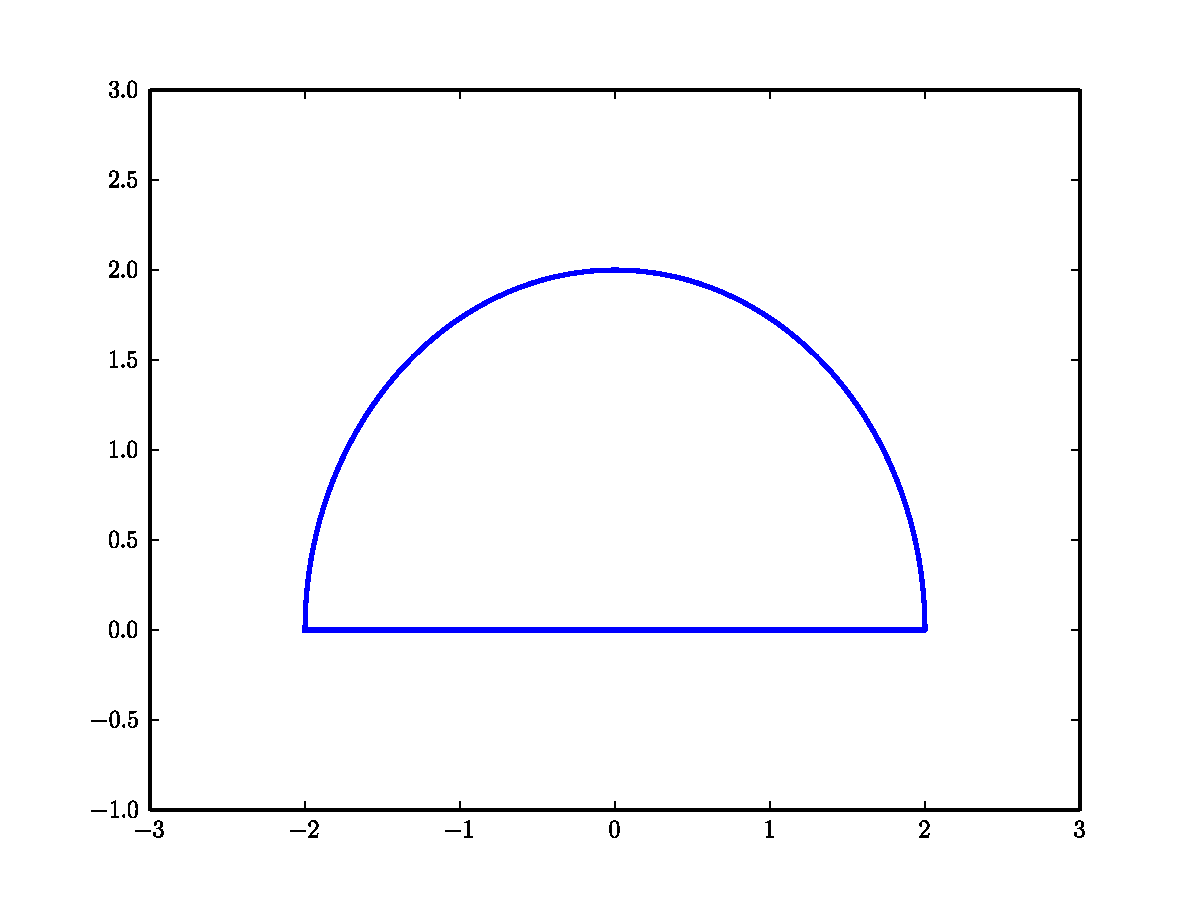
\includegraphics[width=\textwidth]{contour1.pdf}
\caption{A contour used for integration using residues.}
\label{complexint:c1}
\end{figure}

Consider the integral $\int_{-\infty}^{\infty}\frac{z^2}{z^4+1}$. Let $f(z)=\frac{z^2}{z^4+1}$.
Notice that this function has poles at $e^{\frac{\pi i}{4}}$, $e^{\frac{3\pi i}{4}}$, $e^{\frac{5\pi i}{4}}$, and $e^{\frac{7\pi i}{4}}$.
For notation, let these be $p_1$, $p_2$, $p_3$, and $p_4$.
For some real $R>1$, consider the contour $C$ from $-R$ to $R$ and counterclockwise along the circle centered at $0$ of radius $R$ back to -$R$.

This contour ( a semi circle) is shown in Figure \ref{complexint:c1} with $R = 2$.
Let $A$ be this second portion of $C$.
Note that, since $R>1$ we have
\begin{equation*}
\int_C f(z)dz = 2\pi i (\Res{z=p_0} f(z) +\Res{z=p_1} f(z))
\end{equation*}
So, rewriting, we have
\begin{equation*}
\int_{-R}^R f(z) dz = 2\pi i (\Res{z=p_0} f(z) +\Res{z=p_1} f(z)) - \int_A f(z) dz
\end{equation*}
so
\begin{equation*}
\int_{-\infty}^{\infty} f(z) dz = \lim_{R\to \infty} \int_{-R}^R f(z) dz = 2\pi i (\Res{z=p_0} f(z) +\Res{z=p_1} f(z)) - \lim_{R\to \infty} \int_A f(z) dz
\end{equation*}
We would like to show that that $\lim_{R\to\infty} \int_A f(z) dz = 0$, so note that on $A$, $\abs{z}=R$.
It follows from the triangle inequality that $\abs{z^4+1}\geq \abs{\abs{z}^4-1} = R^4 -1$, so we have that 
$$\abs{\int_A f(z) dz}\leq \int_A \abs{f(z)} dz \leq \int_A \frac{R^2}{R^4 -1}dz = \pi R \frac{R^2}{R^4-1}$$
so $\lim_{R\to\infty} \int_A f(z) dz = 0$ as desired.
This then implies that 
\begin{equation*}
 \int_{-\infty}^{\infty} f(z) dz = 2\pi i (\Res{z=p_0} f(z) +\Res{z=p_1} f(z))
\end{equation*}
Evaluating the residues at $p_0$ and $p_1$ we have
$$\int_{-\infty}^{\infty} f(z) dz = \frac{\pi}{\sqrt{2}}$$

\begin{problem}
Write a python function which, given the coefficients for the polynomials in the numerator and denominator of a rational function $f$, evaluates the sum
\begin{equation*}
\sum 2\pi i (\Res{z=p} f(z))
\end{equation*}
over all poles $p$ of $f$ such that $Im(p)>0$.
Use that function to numerically evaluate the following integrals.
$$\int_{-\infty}^{\infty} \frac{z^2}{z^6+1}dz$$
$$\int_{-\infty}^{\infty} \frac{z^{12}-5z^{10}+3z^8-16z^6+4z^4-z^2-4}{4z^{14}+6z^6+12}dz$$
\end{problem}

\begin{problem}
Similar arguments can be used to evaluate integrals of functions that can be compared to the rational functions in question.
Write a modified version of the function you just wrote and use it to evaluate the following integrals.
$$\int_{-\infty}^{\infty}\frac{cos(z)}{z^4+1}dz$$
$$\int_{-\infty}^{\infty}\frac{sin^2(z)}{z^{20}+1}dz$$
\end{problem}

The general conditions in which we may apply this particular way of evaluating integrals come from Jordan's Lemma, which states
\begin{lemma}[Jordan's Lemma]
If for some $f(z)$ on $\mathbb{C}$, $f$ is analytic for all points $z$ in the upper half plane such that $\abs{z}>R_0$ for some $R_0 \in \mathbb{R}$ where $R_0 >0$ and that, where $C_R$ denotes the semicircle $z=Re^{i\theta}$ for $0\leq \theta \leq \pi$, there exists some positive constant $M_R$ such that for all $z$ on $C_R$, $\abs{f(z)} \leq M_R$ and $\lim_{R \to \infty} M_R = 0$, then for every positive constant $a$, we have
$$\lim_{R \to \infty} \int_{C_R} f(z) e^{iaz} dz = 0$$
\end{lemma}
\begin{problem}
Use the function you just wrote to evaluate the Cauchy Principal Value of the integral
$$\int_{\infty}^{-\infty} \frac{z sin(z)}{z^2+1}$$
\end{problem}

If a function has a singularity on the real line, we can often still evaluate the value of $\int_{-\infty}^{\infty} f(z) dz$ using a similar argument as before, but by indenting the path along the real axis around a small path around the singularity, then, as we take the limit as our outer contour moves out toward infinity, we can let the small contour around the singularity approach the singularity.
An example of a contour like this is shown in Figure \ref{complexint:c2}.
It is centered at the origin with $R=2$ on the outer circle and $R=\frac{1}{2}$ on the inner circle.

\begin{figure}
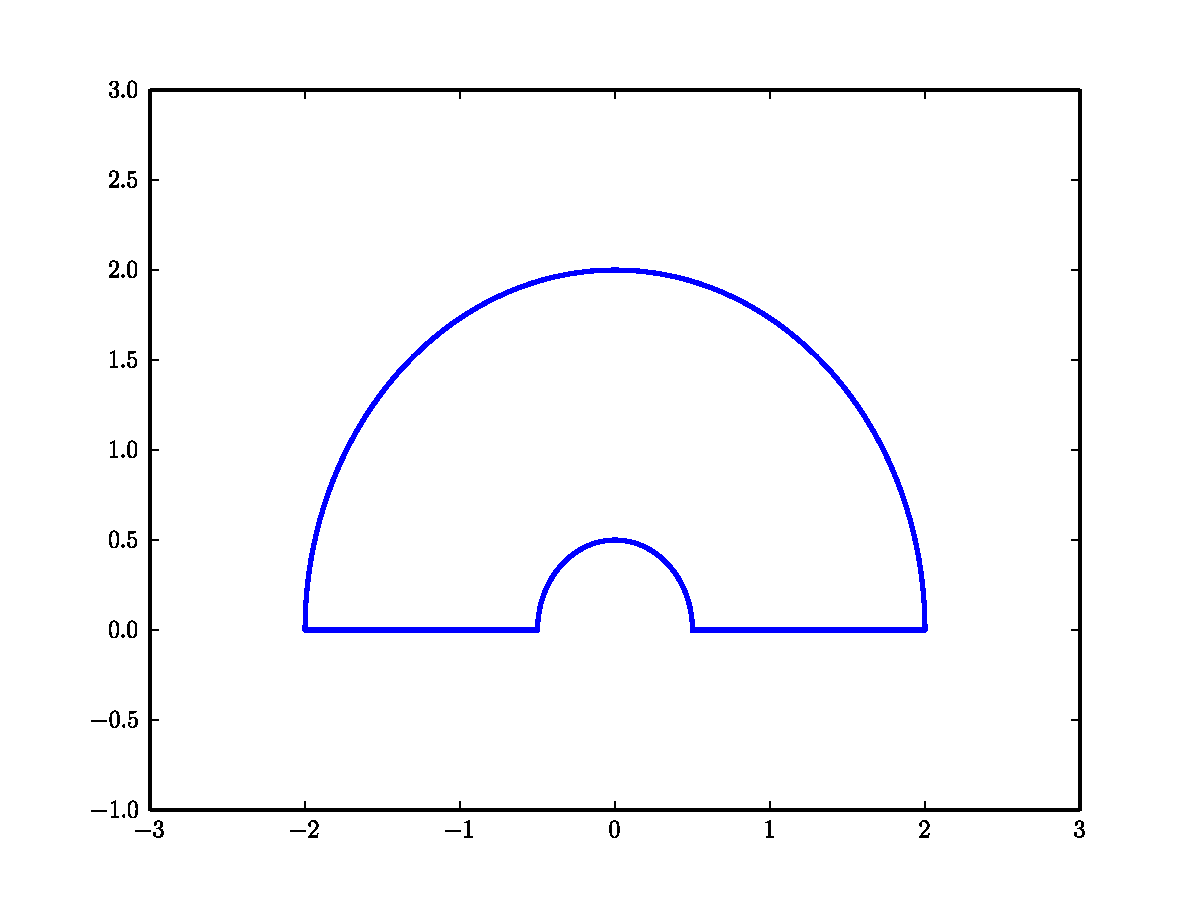
\includegraphics[width=\textwidth]{contour2.pdf}
\caption{An example of a contour that has been modified to avoid a singularity along the real line.}
\label{complexint:c2}
\end{figure}

The following is a useful theorem involving these ``indented path" methods.
\begin{theorem}
Consider a function $f$ with a pole of order $1$ at $z=x_0$ with a Laurent series representation in a punctured disk of radius $R$ about $x_0$ and residue $B_0$ at $x_0$.
Let $C_r$ be the upper half of a circle $\abs{z-x_0}=r$ where $r<R$ oriented in the clockwise direction, then
$$\lim_{r\to 0} \int_{C_r} f(z) dz = - B_0 \pi i$$
\end{theorem}
As a consequence of this, for a function $f$ on $\mathbb{C}$ with only zeros of at most order $1$ on $\mathbb{R}$, where $A$ is the sum of the residues of $f$ on the upper half plane and $B$ is the sum of the residues of $f$ on $\mathbb{R}$, 
$$CPV = \int_{-\infty}^{\infty} f(z) dz = \pi i (B+2A)$$ 
When that Cauchy Principal Value exists.

\begin{problem}
Modify the function you wrote earlier to evaluate the CPV of $\int_{-\infty}^{\infty} f(z) dz$ for a meromorphic function $f$ where $f$ has only poles of order $1$ along the real axis.

Then, using the function you just wrote, evaluate
$$\int_{0}^{\infty} \frac{sin(z)}{z} dz$$

Hint: Since $1/z$ and $sin(z)$ are odd, $\frac{sin(z)}{z}$ will be even, so 
$\int_{-\infty}^{\infty} \frac{sin(z)}{z} dz = 2 \int_{0}^{\infty} \frac{sin(z)}{z} dz$.
\end{problem}

%% Add example 

Integration techniques using residues can also be extended to integration around branch points, some types of integrals involving sines and cosines, inverse Laplace transforms, and many other difficult integration problems.
